\documentclass[10pt]{scrartcl}
% \documentclass[10pt]{article}
\usepackage[T1]{fontenc}
\usepackage{amsmath,amsfonts,amssymb}
\usepackage{mathtools}
\usepackage{color,soul}
\usepackage{fullpage}
\usepackage{enumerate}
\usepackage{graphicx}
\usepackage[colorlinks=true,urlcolor=blue]{hyperref}
\usepackage{caption}
\usepackage{subcaption}
\usepackage{deluxetable}

\definecolor{Light}{gray}{.90}
\sethlcolor{Light}

\title{Some Notes on Albert's Code}
\author{Jeren Suzuki}
\date{Last Edited \today}

\begin{document}

\maketitle
\pagenumbering{Roman}
\tableofcontents
\clearpage
\pagenumbering{arabic}

\section{Introduction} % (fold)
\label{sec:introduction}
Using Albert's C++ as a guide, I've integrated a few of his procedures into IDL. One of the major improvements was the fiducial-finding software. Instead of using two edge-detection filters, we instead use a single convolution filter and check local maxima, then fit them to a parabola for a sub-pixel centroid. 
% section introduction (end)

\section{Rough Center vs Sub-Pixel Center} % (fold)
\label{sec:rough_center_vs_sub_pixel_center}
If we fit a parabola to the local maxima, we can get sub-pixel values for the center, although their accuracy is questionable. See Figure \ref{questionable}. The location of the fiducials just happen to be directly over the pixels so it looks like the not-sub-pixel-method is better, but we need some other solar images to test it on. 

\begin{figure}[!ht]
    \centering
    \hspace{-1.0in}
    \begin{subfigure}[b]{.45\linewidth}
        \centering
        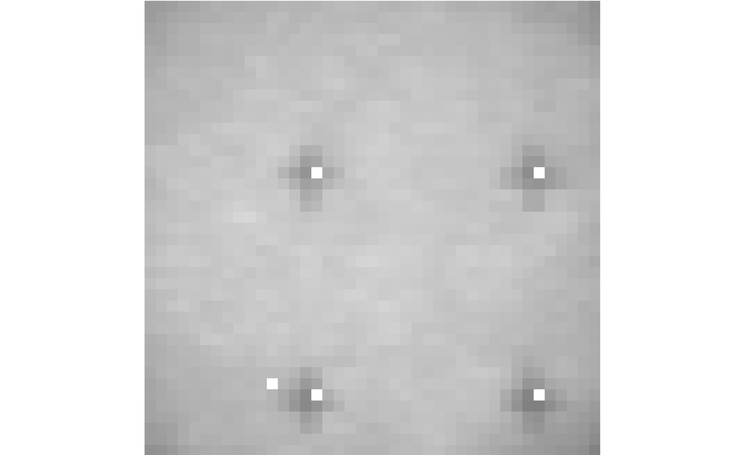
\includegraphics[width=1.3\textwidth]{../plots_tables_images/notsubpix.png}
        \caption{The center of the convolution filter's local maxima}
    \end{subfigure}
    \hspace{.5in}
    \begin{subfigure}[b]{.45\linewidth}
        \centering
        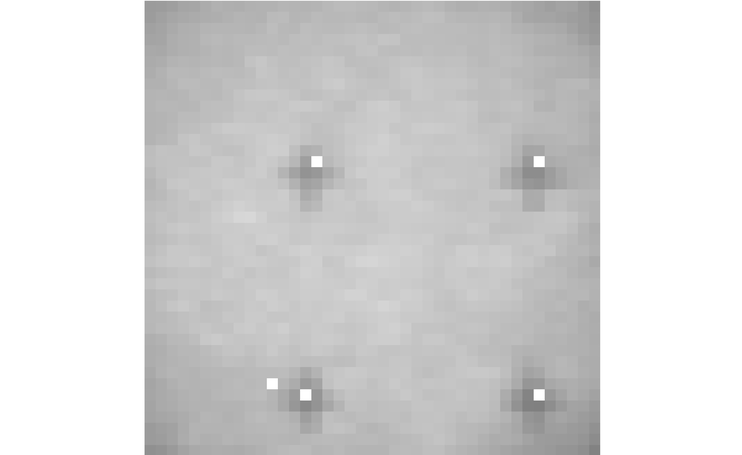
\includegraphics[width=1.3\textwidth]{../plots_tables_images/subpix.png}
        \caption{The center of the parabolic fit to the local maxima.}
    \end{subfigure}
    \caption{Ignore the white pixel near the bottom left fiducial, that is a bright outlier pixel meant for debugging purposes. It is not characteristic to a fiducial.}
    \label{questionable}
\end{figure}
% section rough_center_vs_sub_pixel_center (end)

\section{Information Depth} % (fold)
\label{sec:information_depth}
Albert approaches approximate center-finding in a different way:

\begin{enumerate}
    \item Find pairs of rising/falling edges 
    \item Remove pairs if along fiducial
    \item Remove pairs if too close to limb
    \item Remove pairs if across fiducial
    \item If sun is cut off, create artificial rising/falling edge to force pair
    \item Fit chord edges with a linear fit
    \item Find midpoints of edge-fit chords
\end{enumerate}

There are several major differences than our code. Instead of finding N chords centered around the known approximate center, the chords are made at n\_pix intervals in the entire solar cropped image. This incorporates the need to check if the chord is too close to a limb, which is a step we don't have. The choice of a linear fit instead of a 2nd order polynomial is probably for the sake of speed. \\

Albert's code takes into account the scenario where the sun may be cropped out of part of our image. Our current approach is to use the approximate masking method to find the rough center and leave it at that. We don't use the chord-centering approach if the sun we are looking at is cut off. Not sure if we need to add this condition in our code, but it should be noted.\\

Albert chooses to remove the chords if they are too close to a fiducial, a step that I \emph{should} incorporate rather soonish. The ``problem'' that arises is that since we have a fixed number of chords, removing a chord may be a problem. It will be problematic if, say, we have 5 chords in 1 axis and 2 in another. The chord centers may be biased. Albert's choice to simply remove the chords, however, leads me to believe that this bias is acceptable. 
% section information_depth (end)

\section{Cut off Fiducials} % (fold)
\label{sec:cut_off_fiducials}
The acid test for the new method of centroiding the convolution will be if it can properly detect cut off fiducials. \\

At first, there was a problem with the check-if-your-neighbor-is-higher-than-you part of the code incorrectly finding local maxima strewn throughout the image. The problem was rectified by modifying the threshold value to a stricter value. The result is the fiducial finding code requires 5 fiducial pixels to be inside the image, but other than that, it robustly finds them. See Figure \ref{ohyeah}.

\begin{figure}[!ht]
    \centering
    \hspace{-1.0in}
    \begin{subfigure}[b]{.45\linewidth}
        \centering
        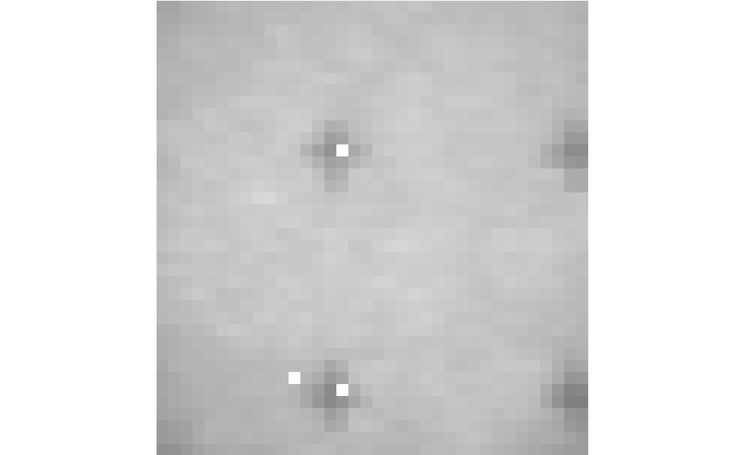
\includegraphics[width=1.3\textwidth]{../plots_tables_images/badcrop.png}
        \caption{The raw image used for fiducual finding} 
    \end{subfigure}
    \hspace{.5in}
    \begin{subfigure}[b]{.45\linewidth}
        \centering
        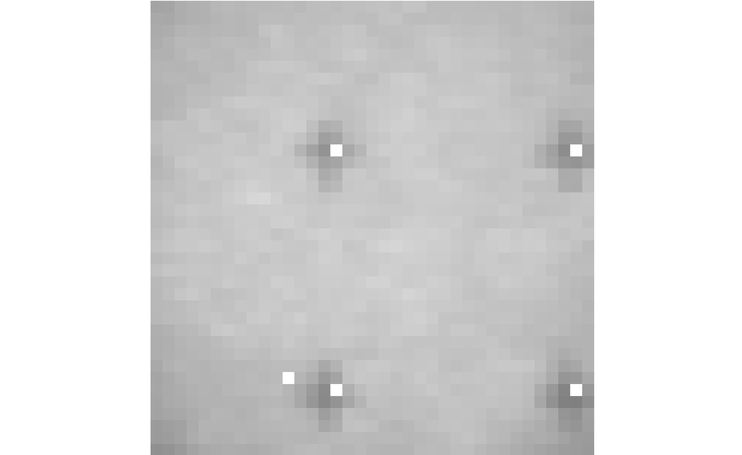
\includegraphics[width=1.3\textwidth]{../plots_tables_images/lessbad.png}
        \caption{If 5 of the 6 fiducial pixels are inside the image, the center is found}
    \end{subfigure}
    \caption{Again, ignore the bright pixel near the bottom left fiducial.}
    \label{ohyeah}
\end{figure}

The convolution filter already has the \hl{\texttt{/edge\_truncate}} keyword to try and deal with edge fiducials and I even tried padding the image but the latter produced some artificial ringing artifacts strewn throughout the image. Hopefully this will be the last we deal of cut off fiducials.

% section cut_off_fiducials (end)

\end{document}










